\documentclass{article}
\pagestyle{plain}

\title{Cache Replacement Policy \\
        \large{Lab2-Advance Memory Systems}}
\author{Ramyad Hadidi}
\date{\today}

\usepackage{graphicx}
\usepackage{amsmath}

\begin{document}

\maketitle

\begin{abstract}
This is the report for Lab2 assignemt for Advance Memory Systems (ECE-7103A) taught by Moinuddin Qureshi on Spring 2015. This assignment is about cache replacement policies. In this assignment three new policies is implemented and their metrics are compared with each other. Also, their results is compared with traditional cache replacement policies like LRU and Random. The policies that are implemented are DRRIP\cite{rrip} and SHiP-PC\cite{ship} plus another replacement policy based on student's preference. These policies are tested with a set of Spec2006 benchmarks. The system for the experiments is a 4-core out-of-order CMP (Chip Multiprocessor) with three level of cache. Our policy is implemented on a 4~MB set-associative Last Level Cache (LLC). The metrics we used are number of misses and Cycles Per Instruction (CPI). The rest of details could be find in the report.
\end{abstract}

\section{Simulation}
Simulation is done with CMP\$im \cite{sim} simulator. Only the source file for cache replacement is modified (\verb+replacement_state.cpp+ and \verb+replacement_state.h+). Simulation is done for a 4-core system which each processor has an 8-stage, 4-wide pipeline. Each processor has its own data and instruction L1 cache. Dcache is 32~KB 8-way set associative with LRU replacement. The L2 data cache is 256~KB, 8-way set-associative with true LRU replacement. The Last Level Cache (LLC) is a 16-way cache with our policy. All simulations in this report are done with 4-threads and 200~M instruction for each. If each thread done its 200~M instruction it will reload its trace again, until all threads are done with their 200~M instructions. In this simulation we \textbf{do not} warm-up the cache. However for the contestant policy in the final section I used 10~M instruction as warm-up.

Table \ref{table_bench} shows our benchmark mixes.

\begin{table}
\centering
\begin{tabular}{|| r | l ||}
  \hline
  Set & Name \\ [0.5ex] 
  \hline \hline
  mcf-mcf-mcf-mcf & mcf \\
  bwaves-bwaves-bwaves-bwaves & bwaves\\
  bzip2-bzip2-bzip2-bzip2 & bzip2 \\
  zeusmp-zeusmp-zeusmp-zeusmp & zeusmp \\
  cactusADM-cactusADM-cactusADM-cactusADM & cactus \\
  hmmer-hmmer-hmmer-hmmer & hmmer \\
  gemsFDTD-gemsFDTD-gemsFDTD-gemsFDTD & gems \\
  sphinx-sphinx-sphinx-sphinx & sphinx \\
  mcf-bwaves-hmmer-sphinx & mix1 \\
  gemsFDTD-bzip2-zeusmp-cactusADM & mix2 \\
  mcf-gemsFDTD-bzip2-cactusADM & mix3 \\
  \hline \hline
\end{tabular}
\caption{Our benchmark in this report \& their names}
\label{table_bench}
\end{table}


\section{Implementation of SHiP-PC \& DRRIP}
We have implemented two policies based on previous papers. The first one is Dynamic Re-Reference Interval Prediction (DRRIP) which is proposed in \cite{rrip}. DRRIP uses set dueling to dynamically choose between Static Re-Reference Interval Prediction (SRRIP) and Bimodal Re-Reference Interval Prediction (BRRIP). In our Implementation we use the Hit Priority(HP) version. In RRIP policy we have M-bit of Re-Reference Prediction Value (RRVP) for each cache line. This value act as a metric for victim selection. A lower value represents a cache line that might be used in near-future. So, in every eviction we choose the line maximum RRVP value (RRIP-MAX) as a victim. In insertion, we insert new line with RRVP value of $RRIP-MAX-1$. In each hit, we improve that line by giving its RRVP a value of zero. Since this report purpose is not describing every detail of the policies we will skip the details.

The second policy is Signature Based Hit Predictor (SHiP)\cite{ship}. In this policy we simply keep a signature for each cache line to represent its behavior. This signature could be PC, memory address or instruction sequence. In order to use less storage, the paper uses hash function to minimize storage overheads. SHiP is the same as SRRIP, however on misses if it finds the line in its table (Signature History Counter Table, SHCT) it will insert with higher priority. In this assignment we have implemented the SHiP-PC which uses PC as lines' signatures.

Table \ref{defines} shows our parameters setups for my SHiP-PC and DRRIP simulations. In section \ref{results} we will compare the metrics for all the policies.

\begin{table}
\centering
\begin{tabular}{ c | l }
  Parameter & Value \\ [0.5ex] 
  \hline \hline
  Number of Leader Sets & 64 \\
  RRVP bits & 2 bits\\
  Dueling Counter bits & 4 bits \\
  Bimodal Insertion Probability & 3.1\% \\
  Number of SHCT entries & $16\times1024$ \\
  Number of Signature bits & 14 bits \\
  SHCT counter bits & 3 bits \\
\end{tabular}
\caption{Parameters for SHiP-PC \& DRRIP}
\label{defines}
\end{table}


\section{Contestant Policy}
I chose Evicted-Address Filter (EAF)\cite{eaf} as my third policy. I tired to mix this idea with RRIP, but the results was not better than ordinary EAF (This is RRIP-EAF in results). In EAF we save the physical memory address of each evicted cache line in a Bloom Filter. Bloom filter acts as a table, but with more less storage overhead. A bloom filter can tell if it has not a value, but it cannot be sure that it has a value in it or not (False Positive). In every miss, if we had that address in our EAF we will insert it as MRU. If not, we will insert it as Bimodal (Always at LRU, on a rare probability at MRU). Figure \ref{pic-eaf} shows this policy.
RRIP-EAF, mix SRRIP policy with EAF. Instead of insert to MRU and LRU positions we insert at RRIP-MAX and RRIP-Max-1. Also, I have implemented the Biomodal policy when we get a miss from EAF, therefore cache will have the chance to adopt to the new workload.

\begin{figure}[h!]
  \label{pic-eaf}
  \centering
    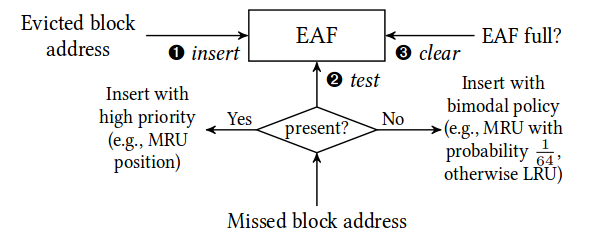
\includegraphics[width=0.7\textwidth]{eaf.png}
    \caption{EAF Mechanism}
\end{figure}

\section{Results} \label{results}
In this section we present our results from different policies. Figure \ref{misses} shows the improvement of number of misses. As it can be seen SHiP-PC gets the best result. The second best policy is could be both EAF version. However, in numbers D-EAF do better. Second graph shows the CPI for different polices for each benchmark. In the end, I have included the exact results in the file attached to this report.

\begin{figure}[h!]
  \label{misses}
  \centering
    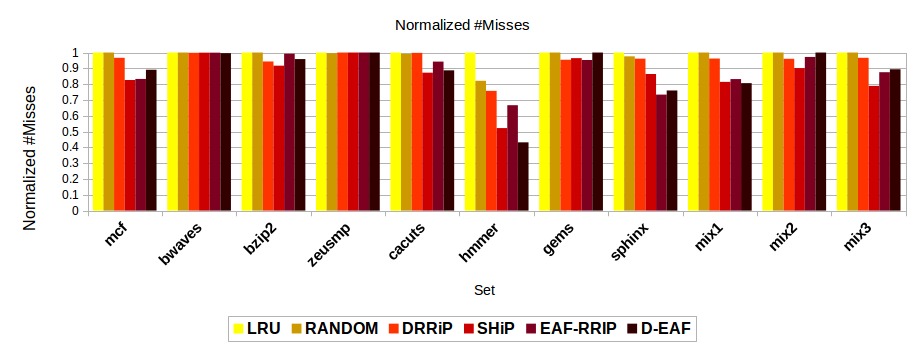
\includegraphics[width=1.0\textwidth]{grap1.png}
    \caption{Normalized Number of Misses}
\end{figure}

\begin{figure}[h!]
  \label{misses}
  \centering
    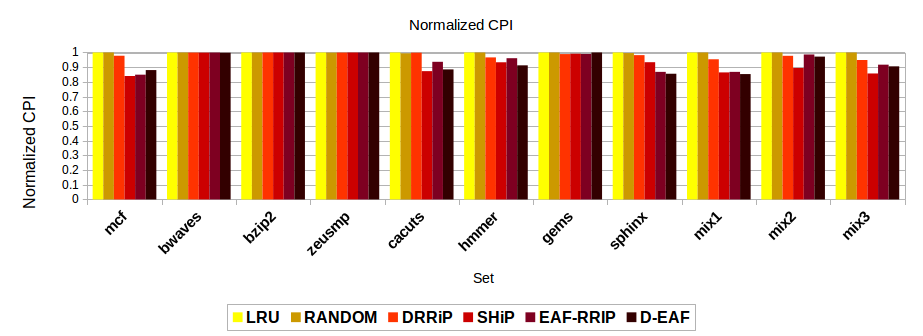
\includegraphics[width=1.0\textwidth]{grap2.png}
    \caption{Normalized CPI}
\end{figure}

\clearpage

\bibliographystyle{plain}
\bibliography{refrences}
\end{document}
